\begin{frame}[t]%
\medskip

\begin{exercise}{Anweisungen}
\begin{body}
Gegeben sei der folgende Ausschnitt eines Java-Programms.
\lstinputlisting[style=JAVAlines]{anweis-2/Anweis2.java}

\begin{parts}
\item[(a)] Welcher Buchstabe wird auf dem Bildschirm ausgegeben, falls \code{i} den Wert $1$, $2$, $3$ bzw. $4$ besitzt?
\item[(b)] Realisieren Sie diesen Programmausschnitt mit einer \code{switch}-Anweisung.
\end{parts}
\end{body}
\end{exercise}

\end{frame}


\begin{frame}[fragile]%
 \frametitle{a) Struktogramm mit Java-Editor}%

\begin{center}
\lstinputlisting[style=JAVAlines]{anweis-2/Anweis2_snippet.java}
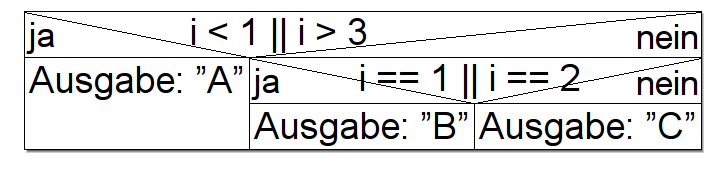
\includegraphics[width=1\textwidth]{anweis-2/Bilder/Struktogramm_a}
\end{center}
\end{frame}


\begin{frame}[fragile]%
 \frametitle{b) Implementierung als \code{switch}-Anweisung}%

\begin{center}
\begin{minipage}{0.7\textwidth}
\codeblock{\noindent
switch ( i ) \{\\
\tab case 1:\\
\tab case 2: \\
\tab \tab System.out.println(''B'');\\
\tab \tab break;\\
\tab case 3:\\
\tab \tab System.out.println(''C'');\\
\tab \tab break;\\
\tab default:\\
\tab \tab System.out.println(''A'');\\
\}
}
\end{minipage}
\medskip

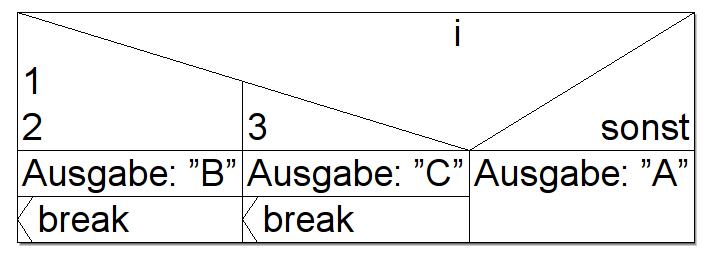
\includegraphics[width=0.8\textwidth]{anweis-2/Bilder/Struktogramm_b}
\end{center}

\end{frame}
